\problemname{Growing Rectangular Spiral}

A growing rectangular spiral is a connected sequence of straight-line
segments starting at the origin. The first segment goes right (positive
$x$ direction).  The next segment goes up (positive $y$ direction). The
next segment goes left (negative $x$ direction).  The next segment goes
down (negative $y$ direction) and the sequence of directions repeats.
Each segment has integer length and each segment is at least one unit
longer than the previous segment.  In the spiral below, the segment
lengths are 1, 2, 4, 6, 7, 9, 11, 12, 15, 20.

% insert image here
\begin{figure}[!h]
    \begin{center}
        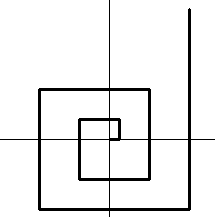
\includegraphics[]{g1.png} \\
    \end{center}
\end{figure}

Write a program to determine the shortest growing rectangular spiral
(in total length) that ends at a given integer point $(x,y)$ in the first
quadrant or determine that there is no such spiral.

\section*{Input}

The first line of input contains a single integer P, ($1 \le P \le 1000$),
which is the number of data sets that follow.  Each data set should be
processed identically and independently.

Each data set consists of a single line of input consisting of three space
separated decimal integers.  The first integer is the data set number.
The next two integers are the $x$ and $y$ coordinates of the desired end point
($1 \le x \le 10000, 1 \le y \le 10000$).

\section*{Output}

For each data set there is a single line of output.  If there is no
spiral solution, the line consists of the data set number, a single
space and \texttt{"NO PATH"} (without the quotes).  If there is a solution,
the line consists of the data set number, a single space, the number of
segments in the solution, a single space, followed by the lengths of the
segments in order, separated by single spaces.  The input data will be
chosen so that no path requires more than $22$ segments.

